\section{Module: aipy.ant}

This module forms the foundation for all modeling, fitting, and simulation code
in AIPY.  Implemented herein are five foundational classes for representing
individual celestial sources, catalogs of sources, antennas, primary beams,
and an entire antenna array.  Other modules will subclass these objects
to add functionality, but these five classes are sufficient to allow
data to be phased to sources.  We will work toward this goal in this chapter.

\subsection{Class: RadioBody (RadioFixedBody, RadioSpecial)}

The goal of the RadioBody is to create an object that can be used for
tracking the position of a source on the sky and projecting baselines in
the direction of that source.  In later modules, this object will be
subclassed to add information about a source's flux and spectral index.
The general functionality of the RadioBody is inherited from the PyEphem
package, which has its own documentation online at 
{\it http://rhodesmill.org/pyephem}.  
RadioBodys come
in 2 flavors: RadioFixedBodys, with fixed celestial coordinates, and
RadioSpecials, which move relative to the celestial sphere.  Generally,
RadioBodys have undefined coordinates until their compute(observer)
method is called on an observer that contains information about latitude, 
longitude, and sidereal time.  Before we can explore RadioBodys
in detail, we will have to create an observer. The most stripped-down 
observer in aipy.ant is the ArrayLocation, which subclasses PyEphem's Observer:

\begin{verbatim}
>>> import aipy
>>> o = aipy.ant.ArrayLocation(location=('40:00:00','123:00:00'))
>>> print (o.lat, o.long), (float(o.lat), float(o.long))
(40:00:00.00, 123:00:00.00) (0.69813170079773179, 2.1467549799530254)
>>> o.set_ephemtime('1980/8/28 12:00') # Set a time in UTC (number or string)
>>> print aipy.ant.ephem2juldate(o.date)
2444480.0
>>> o.set_jultime(2444480.0) # Same thing using Julian dates
>>> s1 = aipy.ant.RadioFixedBody('20:00','40:00',name="CygnusA")
>>> # ra,dec of source can be strings or radians.  Coords in Epoch 2000.
>>> s2 = aipy.ant.RadioSpecial("Sun")
>>> s1.compute(o)
>>> print (s1.ra, s1.dec), (float(s1.ra), float(s1.dec))
(19:59:22.72, 39:57:02.81) (5.2332763671875, 0.6972726583480835)
>>> s2.compute(o)
>>> print (s2.ra, s2.dec), (s2.az, s2.alt)
(1:22:19.41, 8:39:55.77) (298:56:16.64, -18:15:35.20)
>>> print s1.map
[[ 0.84075657 -0.54141333  0.        ]
 [ 0.08157227  0.12667295  0.98858481]
 [-0.535233   -0.83115917  0.15066543]]
\end{verbatim}

Note the fluidity between strings and radians; all string inputs can
equivalently be radians, and radian outputs can print as strings.  You may
be surprised that the right-ascension and declination of s1 weren't what
we set them to--they have been precessed from 2000 to 1980.  In AIPY, 
coordinates are always precessed to the current time.  The Sun (s2) had its 
celestial coordinates computed, even though they are far from static, and
we also demonstrated the availability of observer-centric coordinates
(azimuth = angle clockwise from north, altitude = angle above horizon).
Note that the Sun is not up ($az<0$).  In the last command, we demonstrate that
each source has a matrix for projecting baseline coordinates toward
the source.  We won't need to delve into this though--it will be taken care
of for us under the hood.

\subsection{Class: SrcCatalog}

When there start to be a lot of RadioBodys, it is nice to have a unified
interface for dealing with them.  This will be especially convenient once
we start wanting to sum fluxes and phases over multiple sources.  This
is a relatively simple construct.  Continuing from above:

\begin{verbatim}
>>> cat = aipy.ant.SrcCatalog([s1, s2])
>>> cat.add_src(aipy.ant.RadioSpecial("Moon"))
>>> print cat.keys()
['Sun', 'CygnusA', 'Moon']
>>> o.set_ephemtime("2007/11/20 15:15")
>>> cat.compute(o)
>>> print (cat['Moon'].ra, cat['Moon'].dec), cat['CygnusA'].alt
(0:02:09.15, 2:33:27.7) 11:45:10.4
\end{verbatim}

Observe how calling compute from the SrcCatalog called compute for all
the sources, and that a SrcCatalog behaves as a dictionary indexed by
the names of the sources.

\subsection{Class: Beam}

The Beam class serves two functions.  The first is to model the primary
beam of an antenna element, and the second is to store information about the
observing frequencies.  Since aipy.ant deals only with phasing information
(no fluxes), the primary beam model is not implemented in this base class,
and this Beam serves only the second function.  In greater detail, the
purpose of this Beam is to provide an array (afreq) of the currently
active frequencies (in GHz) to anything that needs to know what frequencies
are to be used in a computation.  It may seem a little ad-hoc for the Beam to 
be the object which carries around this array.  It was chosen for two
reasons: the Beam itself will need to know this information (the primary
beam is always a function of frequency), and everything else (Antennas,
AntennaArrays, etc.) will contain a Beam somewhere.  We'll defer 
Beam examples until the section on AntennaArrays.

\subsection{Class: Antenna}

The Antenna contains all information that is systematic to an element in
an antenna array (i.e. variables that can be solved for by self-calibration).
For the purposes of aipy.ant, this includes physical location (x,y,z),
delay (a phase linearly dependent with frequency), and a phase offset 
(a frequency-independent phase).  Antenna positions are in
nanoseconds (the length of a nanosecond in cgs is defined in aipy.const)
and in equatorial coordinates (x = radial in plane of equator,
y = east, z = north celestial pole).  If you want to convert topocentric
coordinates (in cm) to equatorial coordinates, take a look at aipy.coord.
The delay parameter is in nanoseconds, and offset is in 
$({\rm radians}/2\pi)$.  Again, we'll
defer the tutorial on Antennas until the section on AntennaArrays.

\subsection{Class: AntennaArray (subclassing ArrayLocation)}

Everything comes together in the AntennaArray.  Firstly, it inherits from
ArrayLocation, so you can pass it to the compute() of a RadioBody or
SrcCatalog.  Secondly, an AntennaArray is initialized with a list of
Antennas, and those contain Beams, so an AntennaArrays have all the information
needed to figure out phasing.  Let's learn by example, starting from scratch:

\begin{verbatim}
>>> import aipy, numpy
>>> freqs = numpy.array([.150,.160,.170])
>>> beam = aipy.ant.Beam(freqs)
>>> ants = []
>>> ants.append(aipy.ant.Antenna(0,0,0,beam,delay=0,offset=0))
>>> ants.append(aipy.ant.Antenna(0,100,0,beam,delay=1))
>>> ants.append(aipy.ant.Antenna(100,0,0,beam,offset=.5))
>>> aa = aipy.ant.AntennaArray(ants=ants,location=("18:20:39","-66:45:10"))
>>> print aa.get_baseline(0,2,'r'), aa.get_delay(1,2), aa.get_offset(0,2)
[ 100.    0.    0.] -1.0 0.5
>>> aa.set_jultime(2454447.37472)
>>> srcs = []
>>> srcs.append(aipy.ant.RadioSpecial("Sun"))
>>> srcs.append(aipy.ant.RadioSpecial("Venus"))
>>> cat = aipy.ant.SrcCatalog(srcs)
>>> cat.compute(aa) # REMEMBER to call this before projecting!
>>> print aa.get_baseline(0,1,src=cat['Sun'])
[ 34.66645092 -36.79755511 -86.27964487]
>>> print aa.get_baseline(0,1,src=cat['Venus'])
<class 'aipy.ant.PointingError'>: 'Venus is below horizon'
\end{verbatim}

We made a Beam with frequency information, created 3 Antennas using the
same Beam, and then made an AntennaArray at Arecibo with those Antennas.
We showed how we can access baselines and relative delays and offsets, 
obeying sign conventions depending whether you specify (0,1) or (1,0).  We
made a SrcCatalog containing the Sun and Venus, and then we computed their
locations relative to the AntennaArray. It is important to always call 
compute()
before proceeding to other processing.  At best you will get an error.  At
worst, you could end up with old positions.  Finally, we retrieve baseline
(0,1) projected towards the Sun, and then try to do the same towards Venus.
However, Venus is below the horizon, and rather than let you use a projection
that will give incorrect results, AIPY throws a PointingError.  If you want,
you can catch this exception (aipy.ant.PointingError) and recover.  Note
that the coordinate returned here are still in nanoseconds and are not
yet proper uvw coordinates.  Let's continue:

\begin{verbatim}
>>> print aa.gen_phs(cat['Sun'], 0, 1)
[ 0.26051837-0.96546889j -0.61418129-0.78916496j -0.99988051+0.01545836j]
>>> data = aa.phs2src(numpy.array([.5,1,0j]),cat['Sun'],1,2)
>>> print data
[ 0.44540993-0.22717833j  0.02050412-0.99978977j  0.        -0.j        ]
>>> uvw = aa.gen_uvw(1,2,cat['Sun'])
>>> print uvw
[[  8.86987019   7.55959383  17.72506541]
 [  9.46119487   8.06356676  18.90673644]
 [ 10.05251955   8.56753968  20.08840747]]
>>> print aa.unphs2src(data,cat['Sun'],1,2)
[ 0.5+0.j  1.0+0.j  0.0+0.j]
>>> print aa.rmsrc(numpy.array([.5,1,0j]),cat.values(),1,2)
[ 0.36514582+0.25266785j  0.39471115-0.13255143j  0.12804513-0.41987284j]
\end{verbatim}

Using the AntennaArray and SrcCatalog we created earlier, we can now
use gen\_phs() to return the phases that, when multiplied by data for the
specified baseline, will flatten the fringes of that source.  Note that
3 values are returned here for the 3 active frequencies (we set them
in the Beam).  We could apply these phases to the data ourselves (or
take the complex conjugate and call it simulated data), but 
phs2src() does that for us.  We can also get 
the corresponding uvw coordinates projected toward this source using 
gen\_uvw().  Note again
the 3 entries in uvw for the 3 active frequencies.  To undo what
phs2src() just did, there is unphs2src().  With rmsrc(), we can take a stab
at removing the flux from a list of sources, even though we don't have
any flux information!.  It works by phasing to each source,
taking the FFT to get to lag space, filtering out data around lag 0,
and then unphasing from the source.  For wide bandwidths, this can work
quite well, though in our 3 frequency case it surely does a bad job.

As a final example, we'll process some data in a Miriad file.
For more information about Miriad files, read the
aipy.miriad tutorial.  So that we're working with the same files, run the
following from bash (1 MB download):

\begin{verbatim}
$ wget http://setiathome.berkeley.edu/~aparsons/aipy/test.uv.tar.bz2
$ wget http://setiathome.berkeley.edu/~aparsons/aipy/pwa303.py
$ compress_uv.py -x test.uv.tar.bz2
\end{verbatim}

We're going to make a new file out of test.uv that removes flux from the
Sun and phases to Centaurus A (`cen'), using calibration information from
pwa303.py: 

\begin{verbatim}
>>> import aipy
>>> uvi = aipy.miriad.UV('test.uv')
>>> aa = aipy.loc.get_aa('pwa303',uvi['sdf'],uvi['sfreq'],uvi['nchan'])
>>> print len(aa.ants), aa.get_baseline(0,1)
4 [ 138.14       -222.37112004   -0.70162169]
>>> cat = aipy.src.get_catalog(srcs=['Sun','cen'])
>>> uvo = aipy.miriad.UV('test.uv.mod','new')
>>> uvo.init_from_uv(uvi)
>>> def f(uv,preamble,data):
...     uvw,t,(i,j) = preamble
...     aa.set_jultime(t)
...     cat.compute(aa)
...     data = aa.rmsrc(data, cat['Sun'], i, j)
...     data = aa.phs2src(data, cat['cen'], i, j)
...     return preamble, data
... 
>>> uvo.pipe(uvi, mfunc=f)
>>> del(uvo)
\end{verbatim}

AIPY provides a mechanism (described in greater detail in the tutorial on
aipy.loc)
for defining your own AntennaArray using calibration parameters of your choice
in a self-contained python module.  This module can then be imported into
any script you write, allowing your array calibration to be defined once in
a convenient location, and allowing scripts to be written
that are agnostic about your specific array configuration--they can just
import the appropriate calibration module from the location you specify.
In the above, we opened the Miriad UV file ``test.uv'', and then imported
an AntennaArray containing calibration for this data using get\_aa().
The string ``pwa303'' instructs Python to import the file ``pwa303.py'' using
the default Python module path, which should find the file you just downloaded
in your current directory.
Some additional information is passed to get\_aa() from the UV file regarding
what the channel frequencies are in test.uv. Rather than build up a
SrcCatalog manually, we can ask for a premade one containing specific sources
(or all at once if srcs is not provided) using aipy.src.get\_catalog().
Further information on generating source catalogs is is available in the
tutorial on aipy.src.

Next, we open an output Miriad file (test.uv.mod) for writing and initialize it
with the header information from test.uv.  We define a mapping function that
takes (uv, preamble, data) as an input, and divides the preamble into uvw
coordinates, time (julian date), and baseline indices.  We set the current time
of our AntennaArray, and then call compute() for our SrcCatalog.  We pass our
data through a function that filters out the Sun, and then phase the data to
Centaurus A.  Finally, we return (preamble,data).  All that remains is to pipe
the data through our function.  Because the interactive shell doesn't correctly
destruct objects when it closes, we have to manually delete uvo to close the
file properly.  This is not normally necessary; it is only for the interactive
shell.

To generate a plot of what we did for a single baseline (0,1), run:
\begin{verbatim}
$ plot_uv.py -p yy -a 0_1 -m phs test.uv test.uv.mod
\end{verbatim}

\begin{figure}
\begin{center}
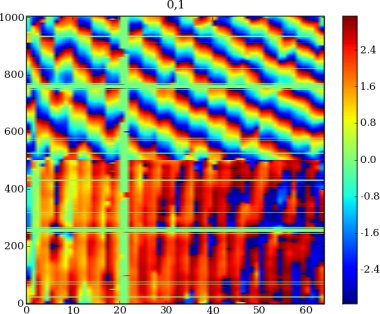
\includegraphics[scale=.5]{plot_test_uv.jpg}
\caption{The vertical axis is time, with test.uv plotted above test.uv.mod.
The horizontal axis is frequency, and the color represents phase.  
Our filtering and phasing removed/flattened the dominant phase in test.uv.
Note that the color blue wraps to red.}
\end{center}
\end{figure}

\subsection{Reference}

\PythonSource*{module_doc/ant.pt}
